\section{Implementation Details}
\label{sec:Solution}
In this section, we describe the system architecture and design choices we made. 

\begin{center}
 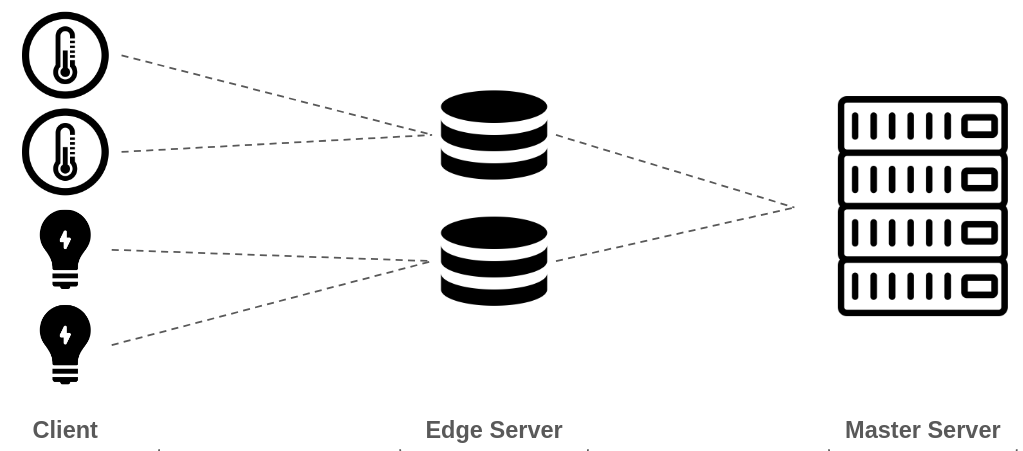
\includegraphics[width=10cm, height=5cm]{sections/Figures/architecture.png}
\end{center}

We implemented the whole project in C++ \cite{prj_git}, but for the evaluation we also implemented a Python version of the client. In the following we explain main components of our system. 
\subsection{Client}
Client send read/write/delete queries to the edge server. In order to improve performance, client put \texttt{write} and \texttt{delete} requests in an ordered queue and sends query request in a batch. This eliminates the redundant write/delete requests on the same key into database. There are two main threads at the client, one for network operations and the main thread. Therefore, the main thread is not blocked during network communication. 

\subsection{Edge Server}
We implemented our own key-value format database which edge-server inherits from. We define three main queries for read, write, and update. Edge server is meant to be close to the clients and we deployed a REST API for connection between clients and edge servers. The main functionality of edge server is to authorize clients and execute their queries on database and return the result. Since we used REST API, we used \texttt{Put} for write query, \texttt{Get} for read query and \texttt{Delete} for delete query.


\subsection{Master Server}
It's important that we guarantee the data persistence among edge servers. We need to make sure if edge servers crashed we don't lose access to it's database; therefore, we also implemented a master server.
Master server receives backup files from the edge servers and store them on a secure, permanent disk storage. Since, there might be a similar key being used by different edge servers, master-server does not translate backup files into a database object and store them as a \texttt{json} file.
